\documentclass[11pt,compress,t,notes=noshow, aspectratio=169, xcolor=table]{beamer}

\usepackage{../../style/lmu-lecture}
% Defines macros and environments
% This file is included in slides and exercises

% Rarely used fontstyle for R packages, used only in 
% - forests/slides-forests-benchmark.tex
% - exercises/single-exercises/methods_l_1.Rnw
% - slides/cart/attic/slides_extra_trees.Rnw
\newcommand{\pkg}[1]{{\fontseries{b}\selectfont #1}}

% Spacing helpers, used often (mostly in exercises for \dlz)
\newcommand{\lz}{\vspace{0.5cm}} % vertical space (used often in slides)
\newcommand{\dlz}{\vspace{1cm}}  % double vertical space (used often in exercises, never in slides)
\newcommand{\oneliner}[1] % Oneliner for important statements, used e.g. in iml, algods
{\begin{block}{}\begin{center}\begin{Large}#1\end{Large}\end{center}\end{block}}

% Don't know if this is used or needed, remove?
% textcolor that works in mathmode
% https://tex.stackexchange.com/a/261480
% Used e.g. in forests/slides-forests-bagging.tex
% [...] \textcolor{blue}{\tfrac{1}{M}\sum^M_{m} [...]
% \makeatletter
% \renewcommand*{\@textcolor}[3]{%
%   \protect\leavevmode
%   \begingroup
%     \color#1{#2}#3%
%   \endgroup
% }
% \makeatother

\newcommand{\open}{}
\newcommand{\close}{}

\title{Interpretable Machine Learning}
% \author{LMU}
%\institute{\href{https://compstat-lmu.github.io/lecture_iml/}{compstat-lmu.github.io/lecture\_iml}}
\date{}

\begin{document}

\newcommand{\titlefigure}{figure/25-05-31_Hooker_2004_graph_fANOVA}
\newcommand{\learninggoals}{
\item Properties of classical fANOVA, reason for its popularity
\item Equivalent definition of classical fANOVA
% \item Understanding why fANOVA theoretically works and what constraints it satisfies
\item Understand the role constraints play for any functional decomposition
}

\lecturechapter{Theory of Standard fANOVA}
\lecture{Interpretable Machine Learning}

\begin{frame}{Example: fANOVA Algorithm}
    \begin{itemize}
        \item Remember: Functional decomposition in general not unique
        \item \textbf{Standard fANOVA} only one possible approach
        \item Example:
        \begin{align*}
            \fh(x_1, x_2) =\,&\,4 - 2x_1 + 0.3 e^{x_2} + |x_1|x_2 \\
            =\,&\,\underbrace{2.95 + 0.3 e.}_{g_\emptyset} + \underbrace{-2x_1 + 0.5|x_1| + 0.75}_{g_1(x_1)} \\
            \,&\,+ \underbrace{0.3 e^{x_2} + 0.5x_2 - 0.3e + 0.05}_{g_2(x_2)} + \underbrace{|x_1| x_2 - 0.5 |x_1| - 0.5 x_2 + 0.25}_{g_{1,2}(x_1, x_2)}
        \end{align*}
        $\leadsto$ seems arbitrarily chosen? \\
        $\longleftrightarrow$ Show: Standard fANOVA fulfills specific desirable properties or \textbf{constraints}
    \end{itemize}

    % See before: The definition of functional decompositions is by far not unique \\

    % BUT: The fANOVA Algo. yields a unique output / unique decomposition, seemingly "arbitrarily chosen".\\

    % \(\rightarrow\) Idea: Uniquely (Eindeutig?) characterize the solution of the fANOVA by its properties. These properties are expressed as mathematical constraints that describe the calculated decomposition.

    % \(\rightarrow\) Two equivalent ways of uniquely / completely defining this decomposition: Either by computation formula defining the single components, or by mathematical equations (the "constraints") defining what properties the components must fulfill
    
\end{frame}

\begin{frame}{Constraints for standard fANOVA Algorithm}

    % One can prove that our definition of the components fulfills the following conditions, called \textit{vanishing condition}:
    \begin{theorem}
    
        Features independent $\implies$ The components defined by standard fANOVA fulfill the so-called \textit{vanishing conditions}:
        \begin{align*}
            \mathbb{E}_{X_j}\left[ g_{S}(\xv_S) \right]
            = \int g_{S}(\xv_S) d \mathbb{P}(x_j) = 0 \quad \text{for any } j \in S \text{ and } S \subseteq \{1, \ldots, p\}
        \end{align*}
    \end{theorem}

    % For independent inputs, the \textit{vanishing condition} is required to obtain a unique solution:
    % $$\mathbb{E}_{X_j} (g_{S}(\xv_S)) = \int g_{S}(\xv_S) d \mathbb{P}(x_j) = 0, \forall j \in S, \forall S \subseteq \{1, \ldots, p\}$$

    % \textit{Proof that our definition fulfills these constraints? Not here}
    
    \pause 
    % Vanishing conditions have the following implications:
    \textbf{Implications:}
    \begin{itemize}
        \item 
        For any component $g_{S}$, all its PD-functions are 0:
        $$
        \mathbb{E}_{X_V}\left[ g_{S}(\xv_S) \right]
        = \int g_{S}(\xv_S) d \mathbb{P}(\xv_V) = 0 \quad \text{for any } V \subsetneqq S \text{ and } S \subseteq \{1, \ldots, p\}
        $$
        $\leadsto$ $g_{S}$ contains no lower-order effects, but only pure interaction term \\
        (compare H-statistic)
        % \item Marginalizing out $x_j, \forall j \in S$ for component $g_S(\xv_S)$ yields a constant 0\\
        % As we integrate out the marginal effect of $x_j, \forall j \in S$ on component $g_S(\xv_S)$ is zero (vanishes)\\
        % $\leadsto$ Makes sure that component $g_S(\xv_S)$ does not contain effects of $x_j, \forall j \in S$
        % For $|S| = 1$ this is equivalent to mean-centering the component $g_S(\xv_S)$. For $|S| > 1$
        \pause
        \item All components are orthogonal, i.e., mutually independent and uncorrelated:
        $$
        \forall V \neq S: \quad \mathbb{E}_{\Xv} \bigl[ g_{V}(\xv_V) g_{S}(\xv_S) \bigr] = 0
        $$
        \item This implies variance decomposition used to define Sobol indices:
    $ \var[ \fh(\xv) ] =  \textstyle\sum_{S \subseteq \{1,\ldots,p\}}  \var \left[ g_{S}(\xv_S) \right]$
    \end{itemize}
    
\end{frame}

\begin{frame}{Examples revisited}
\textbf{Example:} $\fh(\xv) = 2 + x_1^2 - x_2^2 + x_1 \cdot x_2$ (e.g., for $x_1 = 5$ and $x_2 = 10$ we have $\fh(\xv) = -23$)

\begin{itemize}
    \item Computation of components using feature values $x_1 = x_2 = (-10, -9, \ldots, 10)^\top$ gives:
    \begin{columns}[c, totalwidth=\linewidth]
    \begin{column}{0.75\textwidth}
        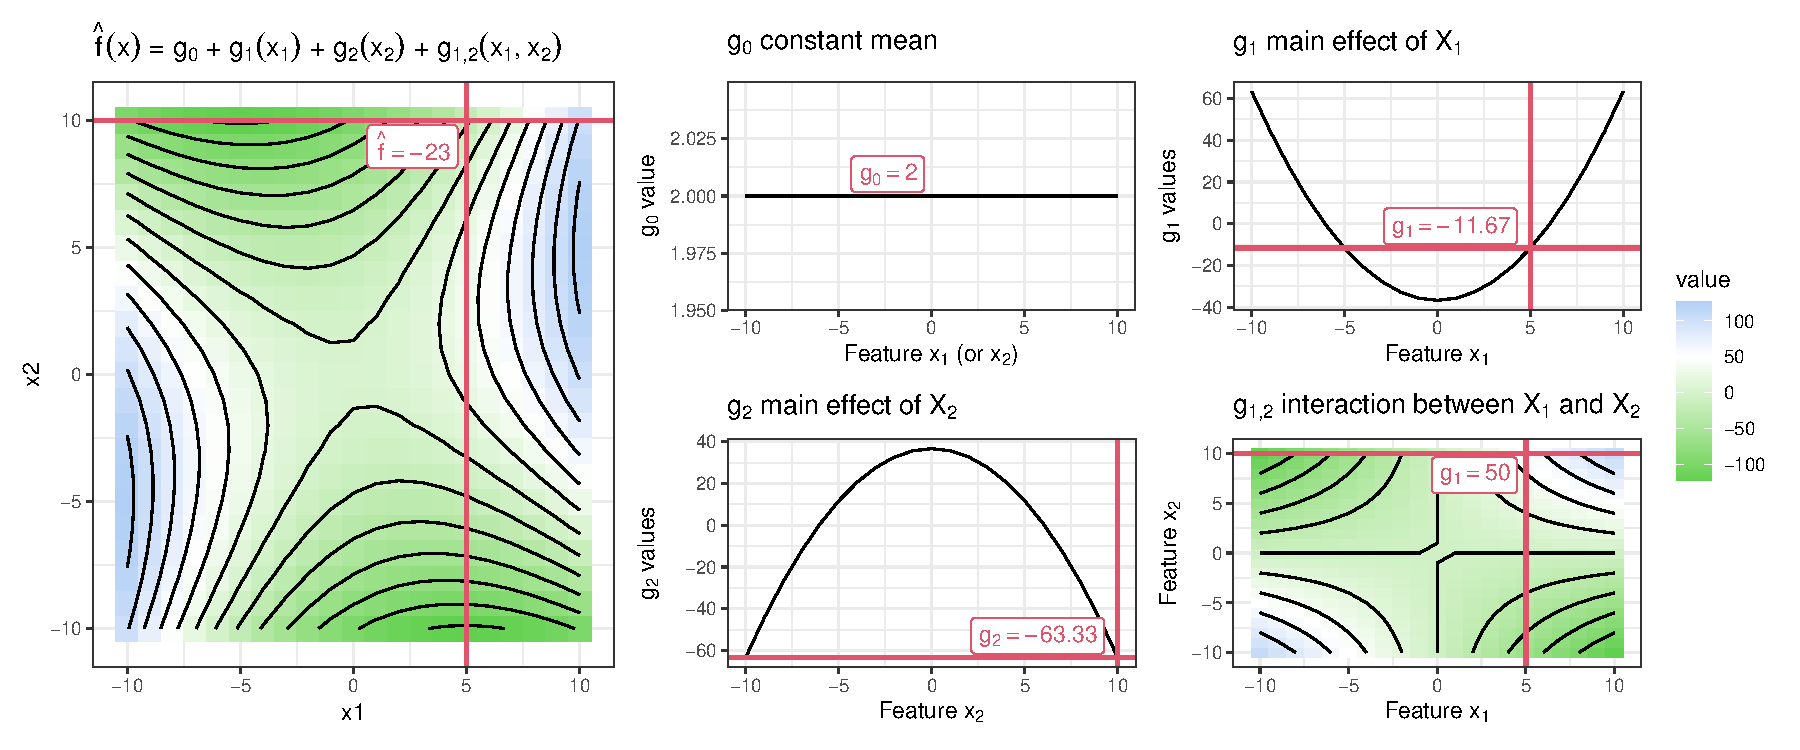
\includegraphics[width = \textwidth]{figure/decomposition}
    \end{column}
    \begin{column}{0.25\textwidth}
    For $x_1 = 5$ and $x_2 = 10$:\\
    \begin{itemize}
        \item $g_{\open \emptyset \close} = 2$
        \item $g_{\open 1 \close}(x_1) = -9.67$
        \item $g_{\open 2 \close}(x_2) = -65.33$
        \item $g_{\open 1,2 \close}(x_1, x_2) = 50$
        \item[$\Rightarrow$] $\fh(\xv) = -23$
    \end{itemize}
    \end{column}
    \end{columns}
% \pause
    \item Vanishing condition means:
    \begin{itemize}
        \item $g_1$ and $g_2$ are mean-centered w.r.t. marginal distribution of $x_1$ and $x_2$
        \item Integral of $g_{1,2}$ over marginal distribution $x_1$ (or $x_2$) is always 0.
        %, i.e., for each slice at $x_1$ (and $x_2$), the integral of $g_{1,2}$ 
    \end{itemize}
\end{itemize} 
\end{frame}

\begin{frame}{Examples revisited}

    \begin{example}
        \begin{align*}
            \fh(x_1, x_2) =\,&\,4 - 2x_1 + 0.3 e^{x_2} + |x_1|x_2 \\
                =\,&\,\underbrace{2.95 + 0.3 e.}_{g_\emptyset} + \underbrace{-2x_1 + 0.5|x_1| + 0.75}_{g_1(x_1)} \\
                \,&\,+ \underbrace{0.3 e^{x_2} + 0.5x_2 - 0.3e + 0.05}_{g_2(x_2)} + \underbrace{|x_1| x_2 - 0.5 |x_1| - 0.5 x_2 + 0.25}_{g_{1,2}(x_1, x_2)}
        \end{align*}
        \begin{itemize}
            \item[$\implies$] Main effect terms inside $g_{1,2}$ are chosen exactly such that the one-dimensional PDPs of $g_{1,2}$ vanish
            \item[$\implies$] Same for constant terms inside $g_1$ and $g_2$: Ensure centering
        \end{itemize}
    \end{example}

    \pause
    \begin{example}
        From in-class exercise:
        $
        g(x_1,x_2)
         = \beta_{12}\,(x_1-\mu_1)(x_2-\mu_2)
        $
    \end{example}
    
\end{frame}

% \begin{frame}{...}

%     [Proofs that these constraints hold / are fulfilled by our definition?? Only briefly]
    
% \end{frame}

\begin{frame}{Constraints: Equivalent characterization}

    \begin{itemize}[<+->]
    
        \item So far: Definition of standard fANOVA implies vanishing conditions
        \item Opposite is true as well: \\
        Features independent $\implies$ Any functional decomposition fulfilling the vanishing conditions must be the standard fANOVA decomposition.
        \item In other words: Vanishing conditions are equivalent characterization
        \item In general: Functional decompositions can be defined by sets of constraints \\
        \item Many other methods to compute decompositions exist, each with their set of constraints
    
    \end{itemize}

    % NB: One can also start the other way around, i.e. define fANOVA using the constraints it should fulfill, and then mathematically prove that the single components must have this form.
    
\end{frame}

% \begin{frame}{Connection to PDP, H-statistics}

%     It can be shown: A PDP for a group of variables is exactly equal to the sum of all fANOVA components which are part of this group.
    
%     The other way round, a fANOVA component can be described as the difference between the respective PDP and all lower-degree PDPs. (plus / minus some other lower-degree PDPs ...)
    
%     Vanishing condition implies: No lower-degree terms / interactions are included in any fANOVA component.
    
%     In general, orthogonality implies that the function contains interactions of a specific type if and only if the corresponding fANOVA component is not 0.
    
%     Together, we achieve an alternative definition / characterization of interactions:
    
%     Interactions of certain type exist \(\iff\) corresponding fANOVA component \(\neq 0\) \(\iff\) the respective difference of PDPs, the so-called \textit{H-statistic}, is \(\neq 0\).

%     More generally, the H-statistic is a measure of the strength of a specific interaction, which can in general be applied to any model or any function.
     
% \end{frame}



\endlecture
\end{document}
